\documentclass[a4paper, twoside]{report}

%% Language and font encodings
\usepackage[english]{babel}
\usepackage[utf8x]{inputenc}
\usepackage[T1]{fontenc}

%% Sets page size and margins
\usepackage[a4paper,top=3cm,bottom=2cm,left=3cm,right=3cm,marginparwidth=2.0cm]{geometry}
\usepackage{parskip} % paragraph style with no indentations and spaces between

%% References
\usepackage[nottoc]{tocbibind} % include bibliography in ToC
\usepackage[numbers]{natbib}
\addto\captionsenglish{
  \renewcommand{\bibname}{References}
} % change name from 'Bibliography' to 'References'

\newcommand{\hlsml}[0]{\texttt{hls4ml} }

%% Useful packages
\usepackage{amsmath}
\usepackage{bm}
\usepackage{graphicx}
\usepackage[table,xcdraw]{xcolor}
\usepackage[colorlinks=true, allcolors=blue]{hyperref}
\usepackage[export]{adjustbox}
\usepackage{adjustbox}
\usepackage{multirow}
\usepackage{xargs}

% Algorithm description
\usepackage{algorithm}
\usepackage{algpseudocode}

%% Itemize lists with more depth
\usepackage{enumitem}
% \usepackage{pifont}
\usepackage{outlines}
\usepackage{amssymb}
\renewcommand{\labelitemii}{$\circ$}
\renewcommand{\labelitemiii}{$\blacksquare$}
% \renewcommand{\labelitemiv}{\textendash}

% Appendix
\usepackage[toc,page]{appendix}

% Clever references from labels
\usepackage{cleveref}


%% Todo notes
\usepackage[colorinlistoftodos]{todonotes} % todo notes, add [disable] to turn them off
\newcommandx{\indo}[2][1=]{\todo[linecolor=red,backgroundcolor=red!25,bordercolor=red,inline,#1]{#2}}
\newcommandx{\maybe}[2][1=]{\todo[linecolor=blue,backgroundcolor=blue!25,bordercolor=blue,inline,#1]{#2}}
\newcommandx{\todofig}[2][1=]{\todo[linecolor=green,backgroundcolor=green!25,bordercolor=green,inline,#1]{#2}}
% \newcommandx{\improvement}[2][1=]{\todo[linecolor=Plum,backgroundcolor=Plum!25,bordercolor=Plum,#1]{#2}}

%% Auxiliary packages
\usepackage{lipsum} % lorem ipsum

\title{Reconfigurable Acceleration of Transformer Neural Networks with Meta-Programming Strategies for Particle Physics Experiments}
\author{Filip Wojcicki}

\begin{document}
\begin{titlepage}

  \newcommand{\HRule}{\rule{\linewidth}{0.5mm}} % Defines a new command for the horizontal lines, change thickness here
  
  %----------------------------------------------------------------------------------------
  %	LOGO SECTION
  %----------------------------------------------------------------------------------------
  
  
\includegraphics[width=8cm]{title/logo.eps}\\[1cm] % Include a department/university logo - this will require the graphicx package
   
  %----------------------------------------------------------------------------------------
  
  \center % Center everything on the page
  
  %----------------------------------------------------------------------------------------
  %	HEADING SECTIONS
  %----------------------------------------------------------------------------------------
  
  \textsc{\LARGE MEng Individual Project}\\[1.5cm] % Name of your university/college
  \textsc{\Large Imperial College London}\\[0.5cm] % Major heading such as course name
  \textsc{\large Department of Computing}\\[1.5cm] % Minor heading such as course title
  
  %----------------------------------------------------------------------------------------
  %	TITLE SECTION
  %----------------------------------------------------------------------------------------
  \makeatletter
  \HRule \\[0.4cm]
  { \huge \bfseries \@title}\\[0.4cm] % Title of your document
  \HRule \\[1.5cm]
   
  %----------------------------------------------------------------------------------------
  %	AUTHOR SECTION
  %----------------------------------------------------------------------------------------
  
  \begin{minipage}{0.4\textwidth}
  \begin{flushleft} \large
  \emph{Author:}\\
  \@author
  \end{flushleft}
  \end{minipage}
  ~
  \begin{minipage}{0.4\textwidth}
  \begin{flushright} \large
  \emph{Supervisor:} \\
  Prof. Wayne Luk \\[1.2em] % Supervisor's Name
  \emph{Second Marker:} \\
  Dr. TODO % second marker's name
  \end{flushright}
  \end{minipage}\\[2cm]
  \makeatother
  
  % If you don't want a supervisor, uncomment the two lines below and remove the section above
  %\Large \emph{Author:}\\
  %John \textsc{Smith}\\[3cm] % Your name
  
  %----------------------------------------------------------------------------------------
  %	DATE SECTION
  %----------------------------------------------------------------------------------------
  \vspace*{\fill}
  {\large \today}\\[2cm] % Date, change the \today to a set date if you want to be precise
  
  \vfill % Fill the rest of the page with whitespace
  
  \end{titlepage}

\begin{abstract}
  Particle Physics studies the fundamental forces and elementary particles building the Universe. In order to verify the correctness of the theories, countless experiments have to be designed and carefully executed, with the main driving force of the myriads of engineers, physicists and researchers at the Large Hadron Collider (LHC) operated by the European Organization for Nuclear Research (CERN). With the unprecedented experiments' scale comes the challenge of accurate, ultra-low latency decision-making. Transformer Neural Networks (TNN) have been proven to accomplish cutting-edge accuracy in various domains, including classification for jet tagging, which is the target of this project. However, software-centered solution implemented for CPUs and GPUs lack the inference speed needed for real-time particle triggers.
  
  This report proposes two novel TNN-based architectures efficiently mapped to Field-Programmable Gate Arrays (FPGAs). The first one outperforms the current state-of-the-art models' GPU inference capabilities by roughly 1000 \todo{Confirm this number} times while maintaining comparable classification accuracy. The second one trades off some of its speed for accuracy and undergoes a broad design-space exploration, which involves both pre-training and post-training quantization. The latter one leverages a custom-developed tool chain that augments existing solutions in terms of granularity and ease-of-use while following an innovative algorithm for relatively quick convergence.

  In this project, several recently researched neural network components are designed to target FPGAs using High-Level Synthesis (HLS). The resulting open-sourced building blocks are both highly customizable and abstract, and aim to bridge the gap between hardware and software development, effectively reducing the time and complexity needed for creating efficient neural network hardware accelerators.
\end{abstract}

\renewcommand{\abstractname}{Acknowledgements}
\begin{abstract}
I would like to express my gratitude to Professor Wayne Luk for his guidance, insightful suggestions and constant encouragement throughout the project.
\newline

I would like to thank Professor Tapper for giving me a different view on the project's meaning and providing with the behind-the-scenes information about the LHC.
\newline

I want to thank Zhiqiang Que for his continuous technical support, our weekly meetings and always being available to answer any of my questions.
\newline

Lastly, I am very grateful for my family whose support was invaluable during this project and the degree as a whole.
\end{abstract}

{\hypersetup{linkcolor=black}
  \tableofcontents
  \listoffigures
  \begingroup % way to display both figure and table lists together
    \let\clearpage\relax
    \listoftables
  \endgroup
}

\chapter{Introduction}

\section{Overview}
Particle physics is one of the key branches of modern physics, with the Standard Model theory at its core. It tackles the underlying questions about the nature of the universe by describing the fundamental forces and elementary particles. In order to verify the correctness of the theories, countless experiments have to be designed and carefully executed, with the main driving force of myriads of engineers, physicists and researchers at Large Hadron Collider (LHC) operated by the European Organization for Nuclear Research (CERN).

LHC is the world's highest-energy particle collider that is capable of producing and detecting the heaviest types of particles that emerge from collisions such as proton-proton collisions. The detection is a challenging process as some particles like quarks and gluons cannot exist on their own, and they nearly instantly combine which results in collimated sprays of composite particles (hadrons) that are referred to as \textbf{jets} \cite{4-cernjets}. The initial particles created upon collision and their behaviors are of main interest of the physicists, which leads to \textbf{jet tagging} - the challenge of associating particle jets with their origin.


\section{Motivation}\label{motivation}
There are many detector types used for the analysis the particle collisions, each based on a different physical phenomenon, which result in availability of both higher and lower level features. The former have been successfully used in the past using more physically motivated machine learning (ML) algorithms, e.g. using computer vision \cite{5-cogan2015jet-images:}. However, more recently, various deep learning approaches have proven to outperform their predecessors \cite{6-de2016jet-images}. It has also been found that all the detected features carry the same underlying information, with convolutional neural networks (CNN) trained on higher-level data achieving nearly identical accuracy as dense neural networks (DNN) trained on the data from the other end of the spectrum \cite{7-moore2019reports}.

The Pb/s throughput of information collected by the LHC detectors outclasses the real-time inference capabilities of the typical state-of-the-art solutions. The real-time decision-making is often required, hence this paper is motivated by the successful adoption of  \textit{\textbf{hls4ml}} codesign workflow in particle physics experiments \cite{8-fahim2021hls4ml:}. It allows ML researchers and physicists to easily deploy their solutions trained using common ML frameworks on reconfigurable or application specific hardware, vastly improving the detection algorithms throughput. However, \textit{hls4ml} lacks support for a number of neural network architectures that have been proven to outperform the previous state-of-the-art, including graph neural networks (GNN) \cite{9-newman2019jedi-net:, 11-elabd2021graph} and transformer neural networks \cite{3-yuan2021constituentnet:}.


\section{Objectives and Challenges}
The purpose of this project is to develop state-of-the-art neural network architectures for Field-Programmable Gate Arrays (FPGA) technology. While working towards this goal, there is an emphasis on creating parametrizable and reusable designs as the next objective is to use metaprogramming strategies to integrate them into the \textit{hls4ml} library with various optimizations that offer trade-offs between speed and hardware resources usage.

The two main challenges of the project involve:
\begin{itemize}
  \item Developing deep and complex neural networks in hardware which requires working at a much lower abstraction level than a typical ML framework. It is also crucial to stay aware of the underlying hardware architecture to exploit its strengths while still making it possible for users' to configure it towards their needs.
  \item Bridging the abstraction gap for the translation between \textit{hls4ml} high-level representation of neural networks and their customizable instantiation in hardware.
\end{itemize}


\section{Contributions}
The project aims to benefit the open-source community of ML researches that are in need of faster and more parametrizable neural network inference. The targeted audience for that operation are physicists at LHC, nonetheless, the hope is for the work to positively contribute in many ML fields by both offering a reliable tool for acceleration of existing designs and providing a useful resource for learning about the nature of reconfigurable hardware and its potential use for neural networks.

\section{Report outline}
This report begins by discussing the necessary particle physics background to understand the scope of the work, followed by the explanation and related work in the field of machine learning, with an emphasis on the state-of-the-art neural networks, and a deeper dive into the reconfigurable hardware technology in \autoref{background}. In \autoref{project-plan} and \autoref{implementation}, the plan for the research is firstly outlined, followed by an up-to-date state of the implementation. Lastly, the planned evaluation metrics are discussed in \autoref{evaluation}, concluded by a consideration of ethical issues that might arise from the work in \autoref{ethical}.

\chapter{Background}

This chapter provides a closer look at the concepts required to understand this work. The following sections firstly discuss background and related work for topics in particle physics, then machine learning and finally reconfigurable hardware research.

\section{Particle Physics}




particle Collisions 
jets
cern
lhc
level x trigger lhc
Physics experiments are crucial
Big data is crucial for Physics


\section{Machine Learning}



training-validation-test dataset
training - 
inference - 
tensor -
machine learning framework
Transformer Neural Networks are great


\section{Reconfigurable Hardware}



c simulation, cosimulation, synthesis

roof ceiling model / pareto front
latency
resource usepackage
throughput
pipelining
HLS
hardware design (parallel vs serial etc)
FPGA are great for NN
FPGA are very hard-coded -> make the code deployable on any platform with optimal settings automatically
HLS is difficult, so coding hardware in Python is desired -> make it easy for engineers and physicists to design systems
Powerful hardware is king
Metaprogramming allows for optimizations and customisability


\chapter{Architecture Exploration}\label{models}
This chapter presents the proposed neural network architectures. It starts with a baseline TNN network implemented in \texttt{PyTorch}, which then undergoes a series of hardware-aware adaptions specific to jet tagging. During this process two separate architectures are developed, which differ by the input type and design goal. The first one, referred to as the \textit{ultra-low latency} one, targets the HLF jet representation and aims to achieve the lowest possible latency at the cost of accuracy and AUC values. The second one, called \textit{accuracy-focused}, is based on the constituent list jet representation and trade-offs latency for quality of classification while still remaining within L1T timing constraints.


\section{Base Architecture}
The starting point of this analysis is derived from transformer architecture used in the original paper \cite{44-vaswani2017attention} and recent proof-of-concept used for jet tagging \cite{3-yuan2021constituentnet:}. The overview of the network components can be seen in figure \ref{fig:constituent-net}.

\begin{figure}[hpt!]
  \centering
  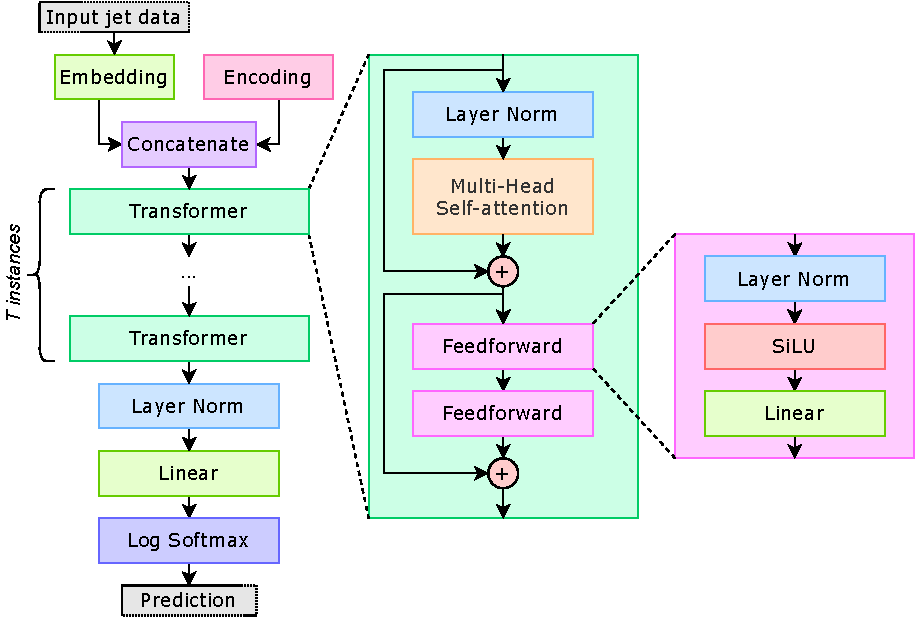
\includegraphics[trim={0cm 0cm 0cm 0cm}, width=0.6\textwidth, center]{models/constituent_net.pdf}
  \caption{Diagram with an overview of the baseline architecture.}
  \label{fig:constituent-net}
\end{figure}

The straight-forward path between model's input and output highlights the sequential nature of transformer which stands in opposition to recurrency present in GRU and LSTM models. While this allows for the aforementioned parallelizability and pipelining on FPGAs, it also poses a challenge of increased hardware footprint and synthesis complexity when compared to recurrent models, where the key components can get reused to meet the resource constraints. To better understand the transformer's complexity, the next subsections derive the equations linking the internal components and explain the involved terminology.


\subsection{Input embedding and Residual Connections}
Although the model lacks any recurrency, the transformer includes two residual connections which have been widely adopted since their successful application in ResNet neural networks \cite{75-kaiming2016deep}. They offer improvements to training time and resulting accuracy \cite{74-szegedy2016inception-v4}, however, they require standardized data dimensionality to ensure the summation can be logically executed. In this project, this is obtained thanks to input embedding, which transforms the input \(\bm{\hat{x^i}} \in \mathbb{R}^{L \times 16} \) into a shape \(\mathbb{R}^{L \times d}\) that is used through the design, as seen in equation \ref{eq:embedding}.

\begin{equation}\label{eq:embedding}
  \bm{\hat{x^i}_{\text{emb}}} = \text{embedding} ( \bm{\hat{x^i}} ) = w_{\text{embed}}\; \bm{\hat{x^i}} + b_{\text{embed}} \in \mathbb{R}^{L \times d}
\end{equation}

This dimensionality change can be conveniently performed using a linear layer, and it has to be remembered that each such layer increased the model learning capacity thanks to the learnable weights and bias. The network's inner dimension \(d\) is treated as a hyperparameter as it influences the model's accuracy and performance, but it has to be noted that the other dimension prevalent in the network comes from the input's number of jet constituents \(L\) (which is set to 1 in case of the HLS representation), meaning that the model is also susceptible to a parameter which cannot be easily tuned.


\subsection{Input Encoding}
Along the embedding, an input encoding is concatenated and fed to the transformer layer. In natural language processing, the encoding is meant to allow the model to benefit from the sequential information of the words in a sentence. It can be obtained from a sinusoidal function using the position index or simply treated as another learnable parameter. The sequential relations are not present in the jet data, because all the jets originate from the same proton-proton collision, hence, the latter approach is used in this project. It is worth mentioning, that from empirical analysis, the learnable encodings have a significant impact on the final results as they represent a trained, hidden state concatenated to all inputs during evaluation, as shown in equation \ref{eq:encoding}. Its impact is especially prevalent for the HLF data (where \(L = 1\)), where the hidden state matched input's dimension and effectively doubles it after concatenation.

\begin{equation}\label{eq:encoding}
  \text{encoding} ( \bm{\hat{x^i}_{\text{emb}}} ) = w_{\text{encoding}} \in \mathbb{R}^{1 \times d} \implies \text{concat} (\bm{\hat{x^i}_{\text{emb}}},\; w_{\text{encoding}}) \in \mathbb{R}^{(L+1) \times d}
\end{equation}

Choosing a learned hidden state is also more efficient for inference in hardware, as the increased training cost associated with back-propagation of this parameter yields a constant set of values that are known during compile-time of the FPGA and can be implemented using a LUT.


\subsection{Normalization and Parameter Extraction}
As layer normalization does not track and gather running mean and variance statistics, this mechanism is implemented on top of the existing \texttt{PyTorch} implementation to facilitate extracting the aggregated statistics after training. These, along with all the learned weights and biases, are extracted and transformed into specific C++ formats supported in HLS using a custom tool developed for this purpose. This allows for directly initializing the FPGA's BRAMs and LUTs with the model parameters, which avoids the need for an interaction with a host machine.

Obtaining the statistics taken for the data before normalization layers can also be viewed as a hardware-aware optimization. This can be explained with the mathematical derivation presented in equation \ref{eq:normalization-optimization}

\begin{equation}\label{eq:normalization-optimization}
  y = \frac{x - E[x]}{\sqrt{Var[x] + \epsilon}} \cdot \gamma + \beta = x \cdot (\frac{\gamma}{\sqrt{Var + \epsilon}}) + (\beta - \frac{\gamma * E}{\sqrt{Var + \epsilon}}) = w \cdot x + b
\end{equation}

By treating the mean \(E[x]\) and variance \(Var[x]\) of input \(x\) as learned parameters, the square root and division operations can be fully omitted by fusing them into the existing \(\gamma\) and \(\beta\) parameters which simplifies the hardware required for the normalization layers. This is especially useful as FPGAs lack dedicated hardware for these computationally expensive operations, which could lead to suboptimal designs being synthesized. Independently of the implementation in this work, a similar idea has been proposed and successfully used as an optimization in the past \cite{46-fan2018real-time}.

The algorithm behind the parameter extraction is rather simple, and the difficulty comes from the domain specific knowledge of handling \texttt{PyTorch} model parameters and generating the correct files for HLS. The break-down of the necessary steps can be seen in algorithm \ref{alg:parameter-extraction}.

\begin{algorithm}
  \caption{Mechanism behind model parameter extraction}\label{alg:parameter-extraction}
  \begin{algorithmic}[1]
    \State $state \gets $load\_state(model)
    \State sort($state$)
    \State $curr\_weight \gets $null
    \For{$param$ in $state$}
      \State $mean \gets $find\_mean(model, param)
      \State $var \gets $find\_var(model, param)

      \If{$param$ is weight}
        \State $curr\_weight \gets $param
        \State $new\_param \gets $update\_weight(param, var)

      \Else
        
        \State $new\_param \gets $update\_bias(param, curr\_weight, mean, var)
      \EndIf
      \State \texttt{save(new\_param)}
    \EndFor
  \end{algorithmic}
\end{algorithm}





\section{Ultra-Low Latency Architecture}
\indo{State the goal and recap the HLF dataset}
\indo{|}

\subsection{Simplification and Tuning}
\indo{List optimizations/simplifications and why they happened, back as much as possible with dataset and being hardware-aware}
\indo{Mention scale changed to shift in self-attention, as explained above}
\indo{|}
\indo{|}
\indo{|}
\indo{|}
\indo{|}

\subsection{Summary}
\indo{Short summary and pointing to diagram}
\indo{|}
\indo{|}

\begin{figure}[hpt!]
  \centering
  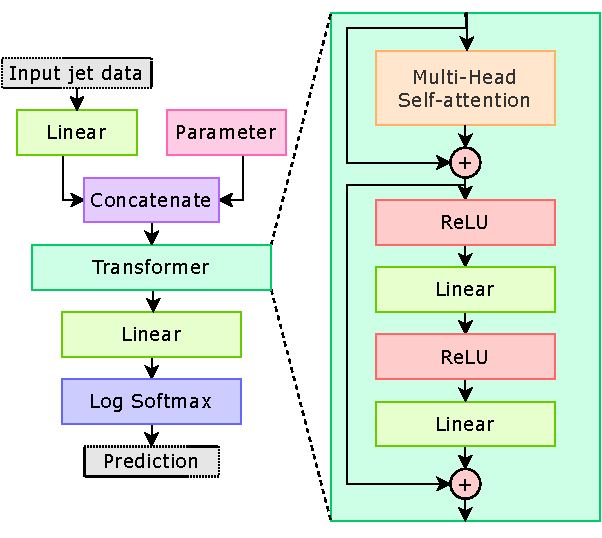
\includegraphics[trim={0cm 0cm 0cm 0cm}, width=0.45\textwidth, center]{models/constituent_net_simplified.pdf}
  \caption{Diagram with an overview of the ultra-low latency architecture.}
  \label{fig:constituent-net-simplified}
\end{figure}


\section{Accuracy-Focused Architecture}
\indo{State the goal and recap the constituent net dataset}
\indo{Talk about big value range of inputs and how we cannot preprocess unless it becomes part of the system (which it does for example to combat numerical instability)}
\indo{Mention how data could be preprocessed in general and reason most methods are too slow/not worth it}
\indo{|}
\indo{|}

\subsection{Simplification and Tuning}
\indo{List optimizations/simplifications and why they happened, back as much as possible with dataset and being hardware-aware}
\indo{stability issues solved by more normalization (coming from wide range of inputs of 30x16)}
\indo{splitting QKV into 3 separate mults}
\indo{|}
\indo{|}
\indo{|}
\indo{|}
\indo{|}

\subsection{Summary}
\indo{Short summary and pointing to diagram}
\indo{|}
\indo{|}

\begin{figure}[hpt!]
  \centering
  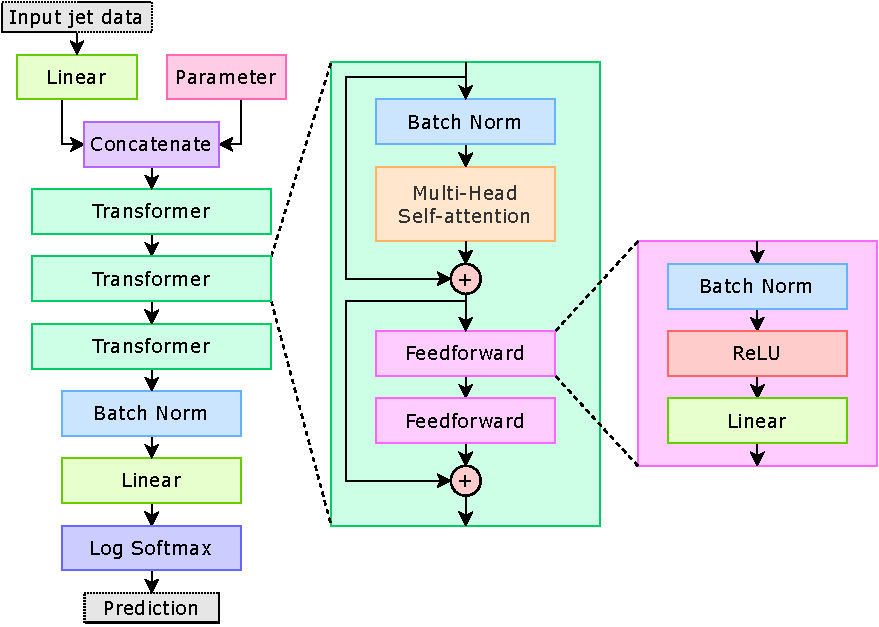
\includegraphics[trim={0cm 0cm 0cm 0cm}, width=0.6\textwidth, center]{models/constituent_net_accuracy.pdf}
  \caption{Diagram with an overview of the accuracy-focused architecture.}
  \label{fig:constituent-net-accuracy}
\end{figure}


\section{Pre-training Quantization}
\indo{Explain what it is and why we do pre-training quantization}
\indo{|}
\indo{|}
\indo{Mention PyTorch Eager Mode and PyTorch FX Graph Mode, give some explanation and show what they can and cannot, overall they are too experimental and cannot support transformer yet}
\indo{|}
\indo{|}
\indo{|}
\indo{|}
\indo{Mention Brevitas, how it compares to PyTorch}
\indo{|}
\indo{Mention QPyTorch, how it compares to PyTorch, Brevitas and why it is the best here}
\indo{|}
\indo{|}
\indo{Mention post-training quantization explained in the next chapter}


\chapter{Hardware Implementation}\label{quantization}
In this chapter, the hardware-aware optimizations used in the FPGA implementations are first presented and then their application in the proposed architectures is explained. Other elements of the hardware design and configuration process are then described which results in a comprehensive picture of the FPGA-mapped architectures. Afterwards, two analytical models are considered - one for the latency and the other for the resource utilization. The custom post-training quantization tool is discussed along with its suitability for this project. Then, existing infrastructure that ties together higher and lower-level code representation is introduced along with its synergy with a High-Level Synthesis optimization tool chain. Lastly, the technical contributions to \hlsml library are listed and explained.

\section{Hardware-Aware Optimizations}

\subsection{Tensor Multiplication and Scaling}
Each self-attention head performs two tensor multiplications (referred to as \textit{matmul} blocks in figure \ref{fig:self-attention-multi-head}), which are normally expressed using Einstein Summation notation \cite{59-barr1991einstein}, which is supported by mathematical and machine learning libraries like \texttt{NumPy} or \texttt{PyTorch}. However, not present by default in HLS, it requires careful design of the calculation loops in order to not cripple the performance by unnecessary computations and pseudo-random data accesses. As part of this research, an efficient and fully-customizable HLS block has been designed, that uses a very similar interface to the Python equivalent.

\begin{figure}[hpt!]
  \centering
  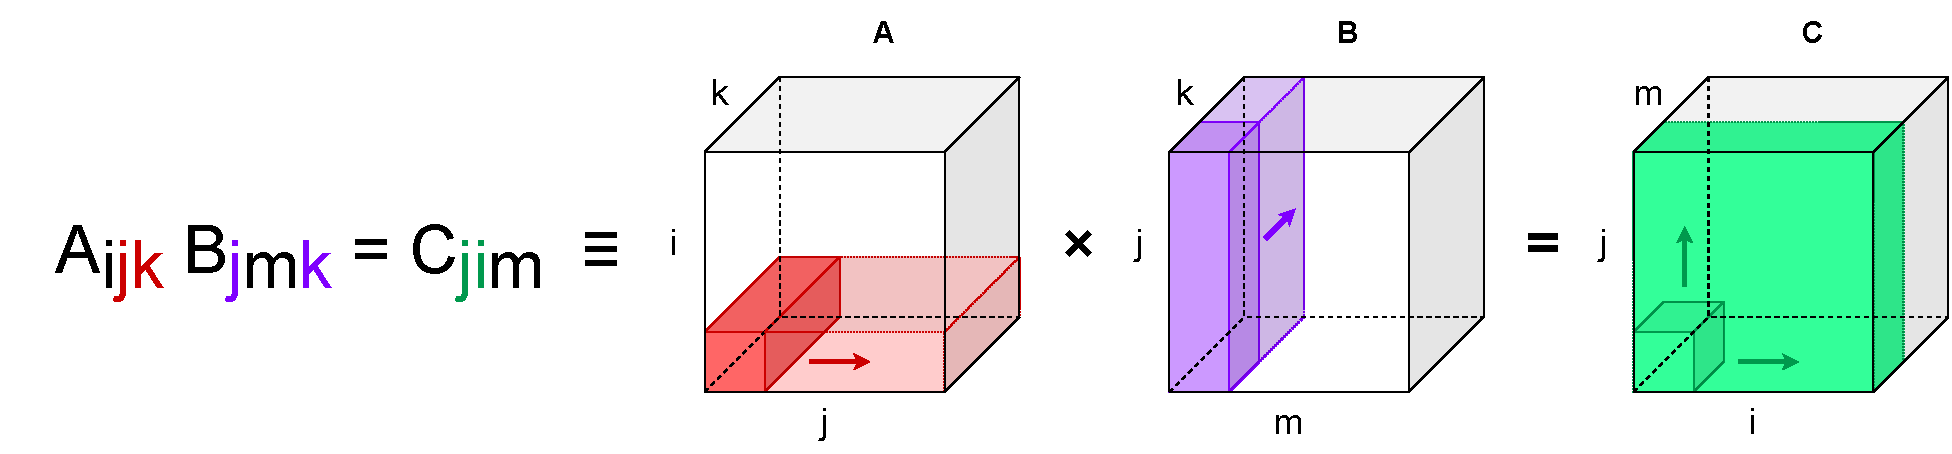
\includegraphics[trim={0cm 0cm 0cm 0cm}, width=0.75\textwidth, center]{models/einsum.pdf}
  \caption{Visualization of a tensor operation expressed in Einstein Summation notation.}
  \label{fig:einsum}
\end{figure}

Figure \ref{fig:einsum} shows a visualization for an example notation to give a better understanding of the necessary flexibility of a formula. The translation between notations using the custom tool is showcased in listing \ref{list:einsum}. While the \texttt{PyTorch} implementation can often use 4-dimensional tensors, the first dimension refers to the batch, which is not present in the hardware implementation that processes input samples one-by-one, hence both the figure and code listing show 3-dimensional cases. It is also worth pointing out, that tensor multiplication is an inherently computationally expensive operation due to the quadruple-nested loop structure. For this reason, the proposed design leaves the configuration of pipelining as a parameter that offers a trade-off between time and design complexity. The \textit{design} complexity refers to the difficulty involved in HLS synthesis as well as hardware resource utilization. In other words, the hardware block can be instantiated to run serially, where little resources are needed as they get re-used, or alternatively, in parallel, where significantly more components are used to decrease latency, and in case the design is also pipelined, to also increase throughput.

% \clearpage
\lstinputlisting[language={[GNU]C++}, caption={From PyTorch \texttt{out = torch.einsum("qhc,khc->hqk", [A, B])} to HLS C++ code.}, captionpos=b, label={list:einsum}]{quantization/einsum_example.cpp}

\begin{equation}\label{eq:einsum-no-unrolling}
  \text{Design}: \mathcal{O}(n) \quad \text{Time}: \mathcal{O}(HKQC \cdot n)
\end{equation}

Let's consider the two extreme cases for the design - no loop unrolling and complete unrolling, where the latter is required for the block to be fully pipelined, and assume that multiply-accumulate and addition both have \(n\) time and space complexity. In the first case, a single multiply-accumulate operation happens at once, hence a final result is only available after all the loops have been fully iterated, with complexities shown in \ref{eq:einsum-no-unrolling}.

\begin{equation}\label{eq:einsum-full-unrolling}
  \text{Design}: \mathcal{O}(HKQC \cdot n) \quad \text{Time}: \mathcal{O}(n \cdot \log (HKQC))
\end{equation}

In the second one, all loop operations can execute at the same time, although the intermediate results need to be summed accordingly using an adder tree (seen in figure \ref{fig:adder-tree}) which has a logarithmic time and linear space complexity, before saving the output tensor, which leads to complexities seen in \ref{eq:einsum-full-unrolling}. The time complexity may appear high, but it has to be remembered that unrolling allows for the pipelining of this design, which cannot decrease latency, but can vastly increase throughput, as each addition can happen in a single cycle.

\begin{figure}[hpt!]
  \centering
  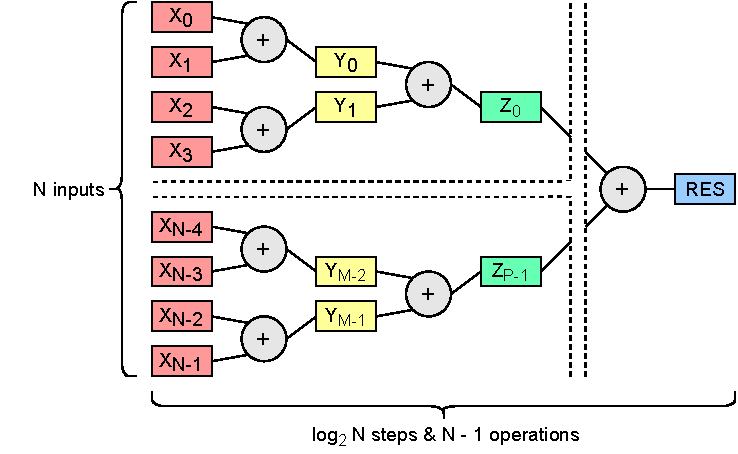
\includegraphics[trim={0cm 0cm 0cm 0cm}, width=0.51\textwidth, center]{quantization/adder_tree.pdf}
  \caption{Illustration of an adder tree with \(N\) inputs.}
  \label{fig:adder-tree}
\end{figure}

Another simple optimization used alongside the tensor multiplication blocks was the change in size scaling from using division to performing an arithmetic right shift (ASR), which requires precomputing the logarithm of the size, seen in equation \ref{eq:log-div}, vastly simplifying the otherwise computationally expensive hardware required at run-time.

\begin{equation}\label{eq:log-div}
  \frac{x}{\sqrt{\text{size}}} \equiv \text{ASR}(x,\; \log_2 \sqrt{\text{size}}) \equiv \text{ASR}(x,\; \frac{1}{2}\log_2 \text{size})
\end{equation}


\subsection{Softmax and Log Softmax Activations}
Despite an already existing \hlsml implementation of the softmax activation function, computing the logarithm of its result is not as simple as it may seem. This is because the numerical stability and computational efficiency of this operation is often explored in-depth \cite{60-blanchard2019accurate} and varies depending on the programming language and target platform.

\begin{figure}[hpt!]
  \centering
  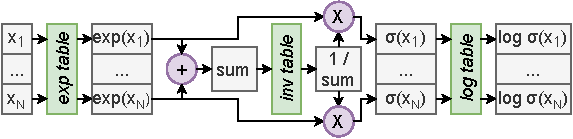
\includegraphics[trim={0cm 0cm 0cm 0cm}, width=0.55\textwidth, center]{quantization/log_softmax_naive_h.pdf}
  \caption{Direct hardware implementations of log softmax.}
  \label{fig:log-softmax-naive}
\end{figure}

The naive implementation comes straight from the definition of taking a logarithm of softmax, seen in equation \ref{eq:softmax}, and the required hardware operations are shown in figure \ref{fig:log-softmax-naive}.

\begin{equation} \label{eq:softmax}
    \sigma (x_i) = e^{x_i} / \sum_{j=1}^{N} e^{x_j}
\end{equation}

This report proposes a different way of mapping this operation to hardware to improve stability while shortening the critical path and using less resources. It is based on the derivation shown in equation \ref{eq:log-softmax}.

\begin{equation} \label{eq:log-softmax}
    \log (\sigma (x_i)) = log(e^{x_i} / \sum_{j=1}^{N} e^{x_j}) = \log(e^{x_i}) - \log(\sum_{j=1}^{N} e^{x_j}) = e^{x_i} - \log(\sum_{j=1}^{N} e^{x_j})
\end{equation}

The resulting hardware operations are depicted in figure \ref{fig:log-softmax-opt}. It is important to note, that operations like exponentiation, division or taking a logarithm usually rely on precomputing a wide range of values and mapping them in BRAMs or LUTs to allow for lookup on run-time. Hence, the optimized design requires one less of such lookups while also replacing multiplication by a subtraction, which can be simpler to express in hardware.

\begin{figure}[hpt!]
  \centering
  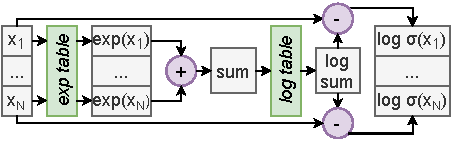
\includegraphics[trim={0cm 0cm 0cm 0cm}, width=0.5\textwidth, center]{quantization/log_softmax_opt_h.pdf}
  \caption{Optimized hardware implementations of log softmax.}
  \label{fig:log-softmax-opt}
\end{figure}

\clearpage
Although further simplifications, including approximating the summation by finding the maximum (see equation \ref{eq:log-softmax-max}) or simply omitting the logarithm portion of the expression, were also explored, they noticeably lowered the final accuracy and were thus abandoned. \todo{Confirm if page breaks correctly.}

\begin{equation} \label{eq:log-softmax-max}
    \log (\sigma (x_i)) = e^{x_i} - \log(\sum_{j=1}^{N} e^{x_j}) = e^{x_i} - \sum_{j=1}^{N} \log(e^{x_j}) = e^{x_i} - \sum_{j=1}^{N} x_j \approx e^{x_i} - \max(x)
\end{equation}


\section{Neural Network Architectures Design}
\indo{|}
\indo{|}
\indo{|}

\subsection{Ultra-Low Latency Architecture}
\indo{|}
\indo{|}
\indo{|}
\indo{|}
\indo{|}
\indo{|}

\subsection{Accuracy-Focused Architecture}
\indo{|}
\indo{|}
\indo{|}
\indo{|}
\indo{|}
\indo{|}


\section{Analytical Latency and Resource Models}
\indo{Reason about computational complexity, include a diagram of self-attention tensor multiplications based on contents of Deep Learning lectures}
\indo{|}
\indo{|}
\indo{|}
\indo{|}
\indo{|}
\indo{|}
\indo{Derive simple latency and resource (likely only DSP as others are too difficult) model, that will be verified in evaluation chapter}
\indo{|}
\indo{|}
\indo{|}
\indo{|}


\section{Post-training Quantization}\label{post-training-quantization}
This section returns to the topic of quantization, but as opposed to \cref{pre-training-quantization}, it explores the quantization of already trained models. This is domain is not researched as much as quantization-aware training due to the lack of ability for a model to \textit{compensate} for the quantization noise during training, hence leading to potentially inferior results. However, recent advancements in this field \cite{80-wang2019haq:} leverage the synergy between post-training quantization and the target hardware platform to produce results with improved latency or energy consumption. The inherent noise issues are offset by a careful per-variable bit-width analysis, driven by a reinforcement learning algorithm. The choice of the algorithm has a deep-rooted issue for more computationally demanding models that also require a search in a wider range of bit-widths\footnote{The mentioned method only explores convolutional neural networks in \([1, 8]\) bit-width range.}.

\subsection{Motivation}
This report proposes a novel post-training quantization algorithm that can be applied to state-of-the-art transformer neural networks over a wide precision range. Early tests in the HLS environment revealed that a single C simulation for an input with only 100 samples can take around 10 minutes, which dictates a need for a significantly simpler, hence faster, algorithm than Bayesian optimization or reinforcement learning to allow for an exploration that runs in a reasonable amount of time.

The motivation of the algorithm comes from a hypothesis which states that the neighboring layers in a neural network have a relatively high correlation in their optimal bit-widths. Under this assumption, each layer's input, output, weight, bias and accumulator can be safely explored one-by-one, in the order of appearance in the model. \textit{Safely} refers here to a low likelihood of arriving at a local accuracy extremum that is substantially worse than the global one, that could only theoretically be found using a more sophisticated approach. During this \textit{walk} through the design space, several non-trivial constraints about the widths have to be ensured, which are the topic of the next subsection.

\subsection{Constraints}
The constraints of a network variable could theoretically be set arbitrarily to convey a high-level requirement of an experienced designer with a knowledge about typical widths used for a component in a given network type. However, the proposed method automates this process by extracting the underlying lookup table characteristics to accommodate users without domain-specific expertise. These characteristics are part of the network configuration that ensures that any precomputed (for increased latency) function is stored with adequate precision that avoids introducing unnecessary errors. To give a more concrete example to this abstract definition, one can consider the range of values yielded from the exponential function. Not only is there a set width for the results, but even relatively small values map to numbers that require several bits of integer precision, so careless reduction to either of the width parts can quickly degrade any learning capacity of the model.

\begin{figure}[hpt!]
  \centering
  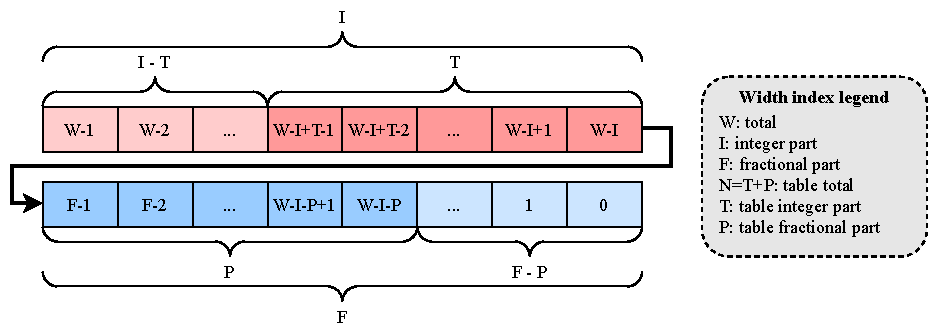
\includegraphics[trim={0cm 0cm 0cm 0cm}, width=1.0\textwidth, center]{quantization/width_constraints.pdf}
  \caption{Visualization of a fixed-point number with its bit-widths as well as constraints imposed by a lookup table. For convenience, red and blue distinguish integer and fractional parts, while the darker hue shows the table-related parts.}
  \label{fig:width-constraints}
\end{figure}

Figure \ref{fig:width-constraints} visualizes a fixed-point number with a detailed analysis of its structure in terms of lookup table constraints. At first, it could be assumed that the imposed widths should simply be adopted by the variables used by the corresponding table values. However, it is possible for such variables to also have connections to other paths in a network, which can require more precision than the table, hence justifying the existence of the constraints ranges presented in equations \ref{eq:width-constraint-1}, \ref{eq:width-constraint-2}, and \ref{eq:width-constraint-3}, with the notation coming from the corresponding figure.

\begin{equation} \label{eq:width-constraint-1}
  W \geqslant N > T \geqslant 1
\end{equation}
\begin{equation} \label{eq:width-constraint-2}
  W \geqslant I \geqslant T \geqslant 1
\end{equation}
\begin{equation} \label{eq:width-constraint-3}
  W \geqslant F \geqslant P \geqslant 1
\end{equation}

\subsection{Steps}



It is important to point out that the aforementioned PyTorch Eager Mode and FX Graph Mode quantization schemes offer post-training quantization, but there are unsuitable for this work due to their lack of flexibility and support for the essential neural network layers.

\indo{Walk through the steps and explain the parameters, pointing to provided algorithm}
\indo{Talk about correlation of neighboring bit widths and how this is exploited (i.e. by resuming with previous width + the whole idea is based on that instead of a full gradient descent style search)}

\begin{algorithm}
  \caption{Algorithm for performing post-training quantization search}\label{alg:post-training-quant}
  \begin{algorithmic}
  \Function{PostTrainingQuantization}{neg\_accuracy\_tolerance, pos\_accuracy\_tolerance}

  \State $previous\_width \gets null$
  \State $max\_decrement \gets neg\_accuracy\_tolerance \cdot 2$ \Comment{Maximum decrement per parameter}
  \State $optimal\_accuracy \gets$ find\_accuracy()
  \State $params \gets$ scan\_file($defines\_file$) \Comment{FIFO with scanned parameter objects}

  \While{$params$ not empty}
    \State $current \gets params$.pop()

    \If{$previous\_width$ exists} \Comment{Try using width from previous parameter}
      \State $original\_width \gets params.width$
      \State update($params$, $previous\_width$)
      \If{find\_accuracy() $< optimal\_accuracy - max\_decrement$}
        \State update($params$, $original\_width$)
      \Else
        \State $optimal\_accuracy \gets$ find\_accuracy()
      \EndIf
    \EndIf

    \For{$part$ in $\{int, frac\}$}

      \State $try\_increase \gets True$
      \State $pos\_improvement\_found \gets False$
      \While{$try\_increase$} \Comment{Increment to check for high accuracy gain}
        \State $param$.increment($part$)
        \If{find\_accuracy() $ > optimal\_accuracy + pos\_accuracy\_tolerance$}
          \State $optimal\_accuracy \gets$ find\_accuracy()
          \State $pos\_improvement\_found \gets True$
        \Else
          \State $try\_increase \gets False$
          \State $param$.decrement($part$)
        \EndIf
      \EndWhile

      \If{not $pos\_improvement\_found$} \Comment{Decrement if no good increment}
        \State $try\_decrease \gets True$
        \State $acc\_before\_decrease \gets optimal\_accuracy$
        \While{$try\_increase$}
          \State $param$.decrement($part$)
          \If{$acc\_before\_decrease -$ find\_accuracy()$ > max\_decrement$}
            \State $try\_decrease \gets False$
            \State $param$.increment($part$)
          \ElsIf{find\_accuracy() $ > optimal\_accuracy - neg\_accuracy\_tolerance$}
            \State $optimal\_accuracy \gets$ find\_accuracy()
          \Else
            \State $try\_decrease \gets False$
            \State $param$.increment($part$)
        \EndIf
        \EndWhile
      \EndIf
    \EndFor
  \EndWhile
  \State \textbf{return} $params$
  \EndFunction
  \end{algorithmic}
\end{algorithm}


\section{High-Level-Synthesis Optimization}
\indo{Introduce MLIR and the overall flow of how PyTorch models are mapped, include nice diagrams}
\indo{|}
\indo{|}
\indo{|}
\indo{|}
\indo{|}
\indo{Talk about how ScaleHLS extends MLIR to HLS, again diagrams}
\indo{|}
\indo{|}
\indo{|}
\indo{|}
\indo{|}
\indo{Talk about potential integration/relation between hls4ml (Python -> HLS) and ScaleHLS (PyTorch/HLS -> Optimized HLS) }
\indo{|}
\indo{|}


\section{\hlsml Contributions}
In this section, the technical contributions to the \hlsml library are descriptively presented, highlighting the areas that this work expands upon. Developed components are shown in figure \ref{fig:hls4ml-contributions}, along with a number of existing components that were expanded upon or are used to draw comparison with. Each group is discussed in the following subsections.

\begin{figure}[hpt!]
  \centering
  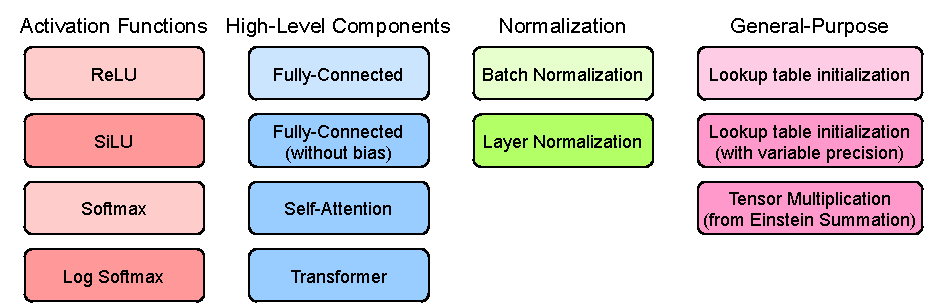
\includegraphics[trim={0cm 0cm 0cm 0cm}, clip, width=0.7\textwidth, center]{evaluation/hls4ml_blocks.pdf}
  \caption{Overview of the created implementations (dark-colored) and some existing components with similar functionality (light-colored).}
  \label{fig:hls4ml-contributions}
\end{figure}


\subsection{Activation Functions}
\indo{Mention SiLU which was experimented with}
\indo{Mention Log Softmax that implements the architecture from previous chapter}
\indo{|}
\indo{|}

\subsection{High-Level Components}
\indo{Briefly mention FC without bias as an optimization that saves initializing accumulators with bias values}
\indo{Talk in details about the C++ HLS challenges and achievements of self-attention and transformer}
\indo{|}
\indo{|}
\indo{|}
\indo{|}


\subsection{Normalization Layers}
\indo{Discuss how layer norm and batch norm actually differ}
\indo{|}
\indo{|}


\subsection{General-Purpose Blocks}
\indo{Explain the mechanism of function look up table initialization and how it was automatic}
\indo{|}
\indo{Show when automatic precision/range fails and how the new block addresses that by exposing int bit width as a parameter}
\indo{|}
\indo{|}
\indo{|}
\indo{Mention tensor einsum and the pragmas it uses}
\indo{|}


% \chapter{Project Plan}\label{project-plan}

The aims of the project cover a wide range of challenges that form the subsequent steps of accelerating neural networks while raising the abstraction layers and reducing domain-specific knowledge requirements. This naturally divides the work into smaller objectives that are described in details in the following paragraphs.

Firstly, the existing transformer neural network architecture has to be redesigned to accommodate for easier adaptation to non-general-purpose hardware. This comprises splitting layers into more basic components that are easier to map to hardware and abstract about as well as introducing hooks that collect different information during training and inference passes (e.g. running mean and variance for normalization layers, tensor sizes and values). At this phase some design choices are highlighted for further inspection where simplification or improvements can be made to greatly reduce the complexity and resource usage without crippling performance.

With the adapted software implementation, the next step involves recreating the architecture in HLS. Building the initial prototype tackles the difficulties related to the underlying differences between software and hardware development and results in an accurate, yet not optimal design. From there, an iterative process begins with acceleration hypothesis firstly tested in the original software model to ensure satisfactory accuracy and then getting expressed in HLS to quantitatively measure the latency and throughput differences. This is expected to yield a highly performant solution to the initial problem that is tailored specifically to the FPGA constraints.

In order to overcome the innate limitations of "hand-tuning" a solution to a problem that varies both in time and between applications, the final step of the project relies on meta-programming strategies that automatically adapt the solution according to users' criteria, available platforms and overall experiment's aim. The list of approaches that can be taken here is nearly endless, however two key areas have been designated - adjusting the model according to the existing hardware to exploit its strengths as well as allowing for more abstract representation of an architecture in a well-known machine learning framework.

As previously mentioned, some initially planned ideas have already been implemented. The distinction between these and a more detailed look at the specific project tasks can be seen in figure \ref{fig:gantt-chart}. It is important to note the project milestones and exam sessions at the bottom of the diagram, as they give a better context of the spread of the working time. Although very time-consuming, coursework deliverables have not been highlighted, as all combined they occur in every week of the Spring term and would introduce too much information clutter.

\begin{figure}[hpt]
  \centering
  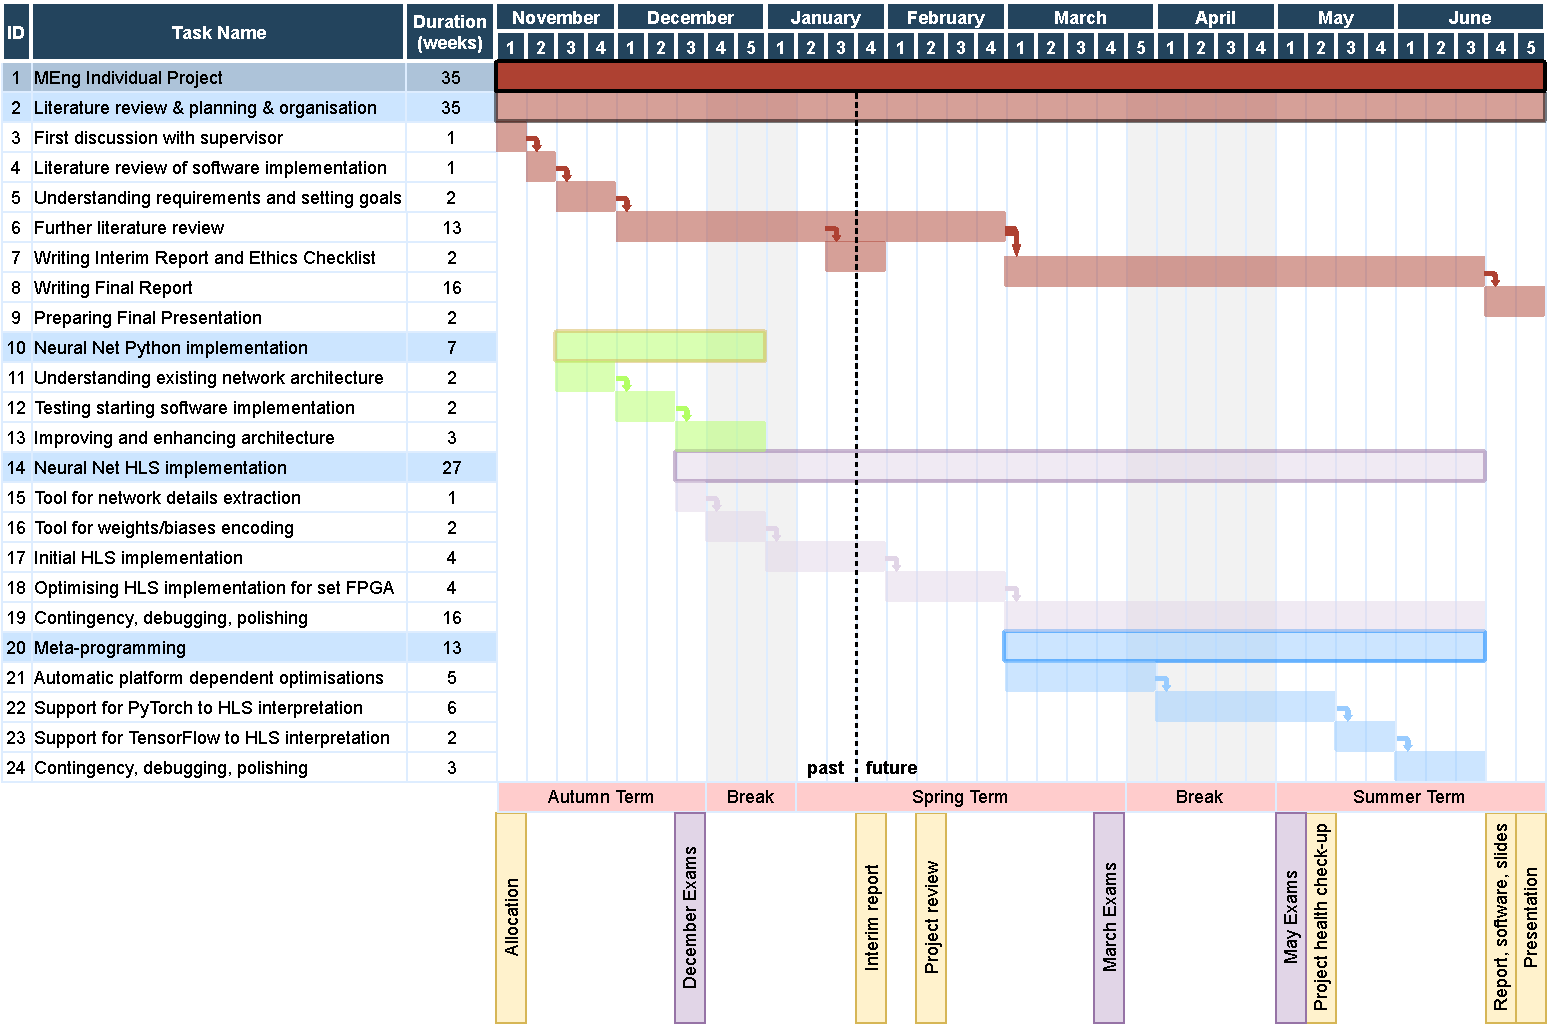
\includegraphics[trim={0cm 0cm 0cm 0cm}, width=1.2\textwidth, center]{project/gantt_chart.pdf}
  \caption{Project's Gantt chart representing initial plan of the work; past schedule has been updated to match ongoing progress accordingly}
  \label{fig:gantt-chart}
\end{figure}
% \chapter{Implementation}
\chapter{Evaluation Plan}

This section outlines the proposed evaluation plan for the project. The first objective of developing and optimizing a state-of-the-art neural network in hardware can be evaluated quantitatively, while integrating it into the \textit{hls4ml} library and making it easy for new users to use requires a more qualitative approach.

\section{Quantitative results}
The following describes the quantities that are planned to be measured:

\begin{outline}
  \1 Classification accuracy for each designed neural network on a validation dataset
  \1 Inference latency and throughput when running on the target platform
  \1 Hardware resource utilization (exact values for comparison with other platforms and percentage of available resources for understanding limitations):
    \2 Block RAM (BRAM)
    \2 Ultra RAM (URAM)
    \2 Digital Signal Processing units (DSP)
    \2 Flip-Flops (FF)
    \2 Look-Up Tables (LUT)
\end{outline}

In the early stages of the project, the above quantities will be measured from the results from simulation and synthesis reports. At a later stage, the best designs will be run on actual hardware platforms to validate them under real-life use cases. The platform planned for this part is an Intel Stratix V FPGA hosted in a Maxeler MPC-X dataflow node with 8 Maia dataflow engines and 48 GB of DRAM.

Apart from clear design improvements, it is predicted that most evaluated designs will offer trade-offs between classification accuracy, inference throughput and hardware utilization. It is not possible to find a design that is superior in every way, hence a \textbf{Pareto front} will play a key role in understanding the overall performance and selecting configuration with specific needs in mind.

\section{Qualitative results}
Qualitative

\chapter{Conclusion}\label{conclusion}
This work provides important insights into reconfigurable acceleration of transformer neural networks for ultra-low latency applications like high energy physics. The proposed solutions cover the whole development spectrum, from software architecture design, through various optimization techniques, to efficient hardware mapping of the neural network models. In this chapter, the main technical contributions are firstly summarized, followed by a discussion covering the existing limitations discovered during our research. Finally, several possible extensions that could improve upon our work are covered.

\section{Achievements}
This project contributes to the following research areas:

\begin{itemize}
  \item \textbf{Hardware-Aware Neural Network Design}: We explore two neural network architectures, which combine ideas from state-of-the-art solutions and transform them into components that can be efficiently mapped to FPGAs while offering cutting-edge accuracy. The analyzed aspects involve weight and bias fusing for normalization, splitting of fully-connected layers, and preventing numerical instability in softmax activation function. To allow for an easier reasoning about the architectures, analytical models covering latency and DSP slices were developed.

  \item \textbf{Efficient Hardware Mapping}: We propose novel hardware blocks for tensor multiplication using Einstein Notation as well as latency and resource optimized log softmax and SiLU activations. On top of that, we further expand \hlsml library with efficient and customizable self-attention and transformer layers. We also introduce improvements to the fully-connected layer and the unit responsible for storing results of arbitrary precomputed functions. The resulting hardware design achieves nanosecond latency with classification quality comparable to GPU and CPU implementations that are run around thousand times slower.

  \item \textbf{Quantization-Aware Training}: We analyze existing solutions for quantization-aware training and adapt the most suitable framework to transformer neural networks. The conducted experiments highlight the best performing fixed-point representations and highlight potential pitfalls in very complex neural networks.

  \item \textbf{Post-Training Quantization}: We develop a novel algorithm for post-training quantization that can be used with existing models and target any hardware platform. Thanks to its user-defined parameters, the search can be configured to prioritize accuracy over resource utilization or vice-versa. Evaluation on the proposed models results in a nearly \nicefrac{2}{3} reduction of total bit-widths with negligible accuracy decrease.
\end{itemize}

\section{Limitations}
Due to the scope of the project, there was no extensive hyperparameter search involved in any of the neural network architectures. Further tuning might allow for better results, which can have a cascading effect on the rest of this report's analysis because the researched areas are tightly coupled. In other words, more optimized software models lead to better performing hardware implementations, which can be further amplified by carefully quantizing them during or after training. On that topic, the developed post-training quantization algorithm assumes high correlation between subsequent neural network layers. Although this was proven to be the case in our analysis, it might not generalize to every network type.

The more complex of the discussed transformer architectures was not able to be synthesized as a pipelined design using HLS due to the inherent intricacy of generating pipelined models. The serial implementation offers an interesting trade-off of a design that runs slower but requires substantially less resources. However, many real-life applications operate under strict latency constraints, which could not be met due to the existing limitations of the HLS process and the fundamental issue of transformer's complexity.

\section{Future Work}
There are four main areas that our work could be expanded upon, which involve modifying the transformer layer, especially the self-attention mechanism, enhancing the post-training quantization method, adapting existing High-Level Synthesis optimization tools, and experimenting with other datasets.

\subsection{Alternative Transformer Design}
There is an ongoing research into alternative transformer architectures, which improve upon the quadratic complexity of self-attention, that has proven to be the main challenge of accelerating transformers. Some solutions involve low-rank approximations, sparsity, memorization, or various other techniques, summarized in figure \ref{fig:transformer-landscape} \cite{81-tay2020efficient}. To tackle the complexity problem, a recent work also goes as far as exploring completely removing the self-attention layer \cite{82-mikuni2021point}.

\begin{figure}[hpt!]
  \centering
  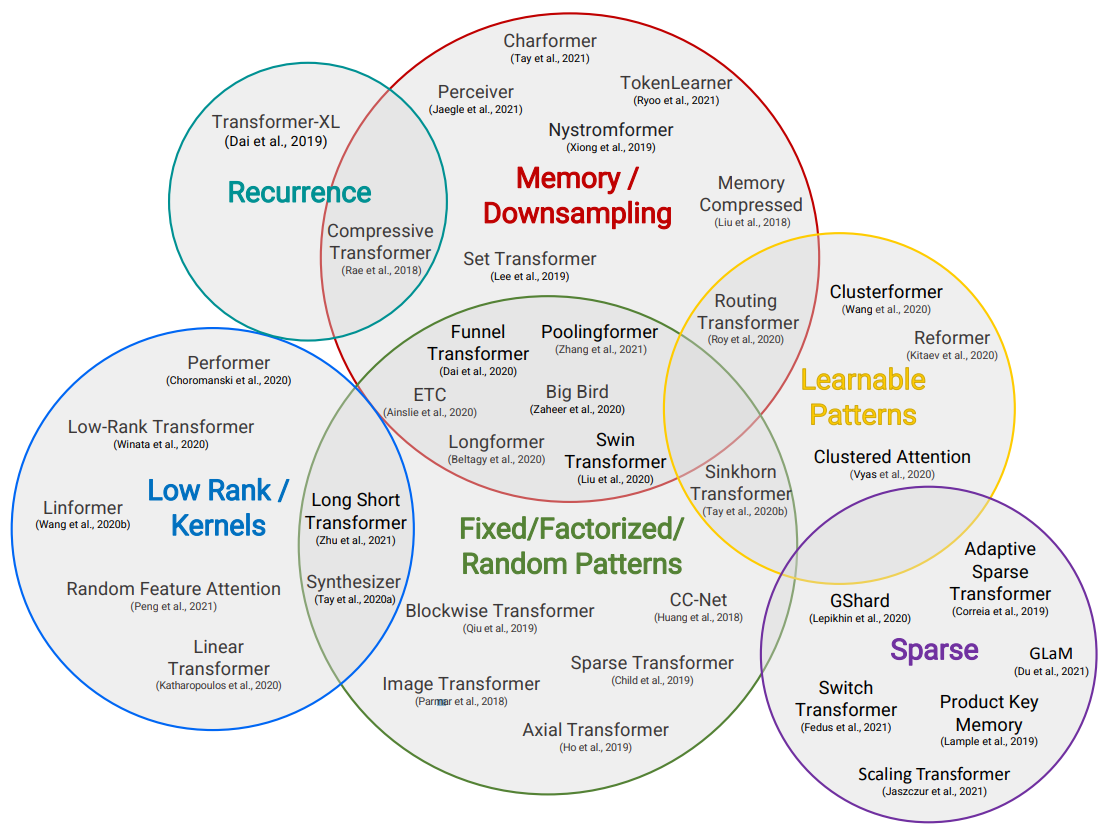
\includegraphics[trim={0cm 0cm 0cm 0cm}, clip, width=0.7\textwidth, center]{conclusion/transformer_landscape.png}
  \caption{Landscape of efficient transformer architectures.}
  \label{fig:transformer-landscape}
\end{figure}

Aside from changes to self-attention, trained transformer models could be compressed using techniques like pruning to decrease the number of stored weights which can improve the inference speed and reduce hardware utilization. Additionally, the already optimized batch normalization layers could be further improved by fusing with linear layers to reduce the overall complexity. Finally, recent automatic methods of finding efficient transformer configurations \cite{83-tsai2020finding,84-su2021vitas:} could help with the hardware-aware architecture search challenge.

\subsection{Post-Training Quantization Advancements}
The proposed post-training quantization algorithm could base its resource estimations on an analytical model to achieve more accurate predictions without compromising the search time. A new metric of energy-consumption could also be taken into consideration to accommodate mobile or embedded platforms' limitations. In order to accelerate the search process while potentially improving its findings, the approach could also benefit from a faster simulation and awareness of tested configurations' positions with regard to the underlying Pareto front or Roofline Model.

\subsection{Automatic High-Level-Synthesis Optimizations}
A recent High-Level Synthesis framework called ScaleHLS \cite{ye2021scalehls} promises to generate efficient RTL designs from HLS C++ or directly from PyTorch thanks to the use of optimizations at different levels of abstraction of the underlying Multi-Level Intermediate Representation (MLIR) \cite{mlir} used for PyTorch \cite{86-llvm2020torch-mlir}. This tool was explored during the project, but similarly to the discussed quantization-aware training methods, it does not support the self-attention layer in case of the direct PyTorch model optimization. As for trying it on the already developed HLS implementation, the size and the deep hierarchy involved in this work exceeds the complexity that ScaleHLS can handle. Nonetheless, further improvements might allow this framework to reduce the development time between designing a transformer architecture using \hlsml and testing its hardware implementation, supporting the objective of this work.

\subsection{Other Datasets}
Both of the datasets used in this project involve classification of five jet categories. However, other examples in the literature often discuss problems with fewer categories, for instance top-tagging, which is an approach to identifying top quarks. Simpler problems are likely to require less complex architectures - an area of the design space that this work proves to be optimal for transformers.

%//////////////////////////////////////////////////////
% at the end, CHECK:
% hyphens,
% 3rd person s in verbs,
% remaining todos,
% ugly page breaks,
% axis and titles in figures,
% correct some references to evaluation to be more specific (find all of them),
% change explanation in (brackets) to footnotes (always?),
% ensure no pre-training quantization but quantization-aware training,
% ensure network names like CNN, TNN are used consistently + no capital letters in convolutional nn, transformer nn,

\bibliographystyle{unsrtnat}
\bibliography{references/references}

\begin{appendices}

\chapter{HLF dataset features distribution}
\begin{figure}[hpt!]
  \centering
  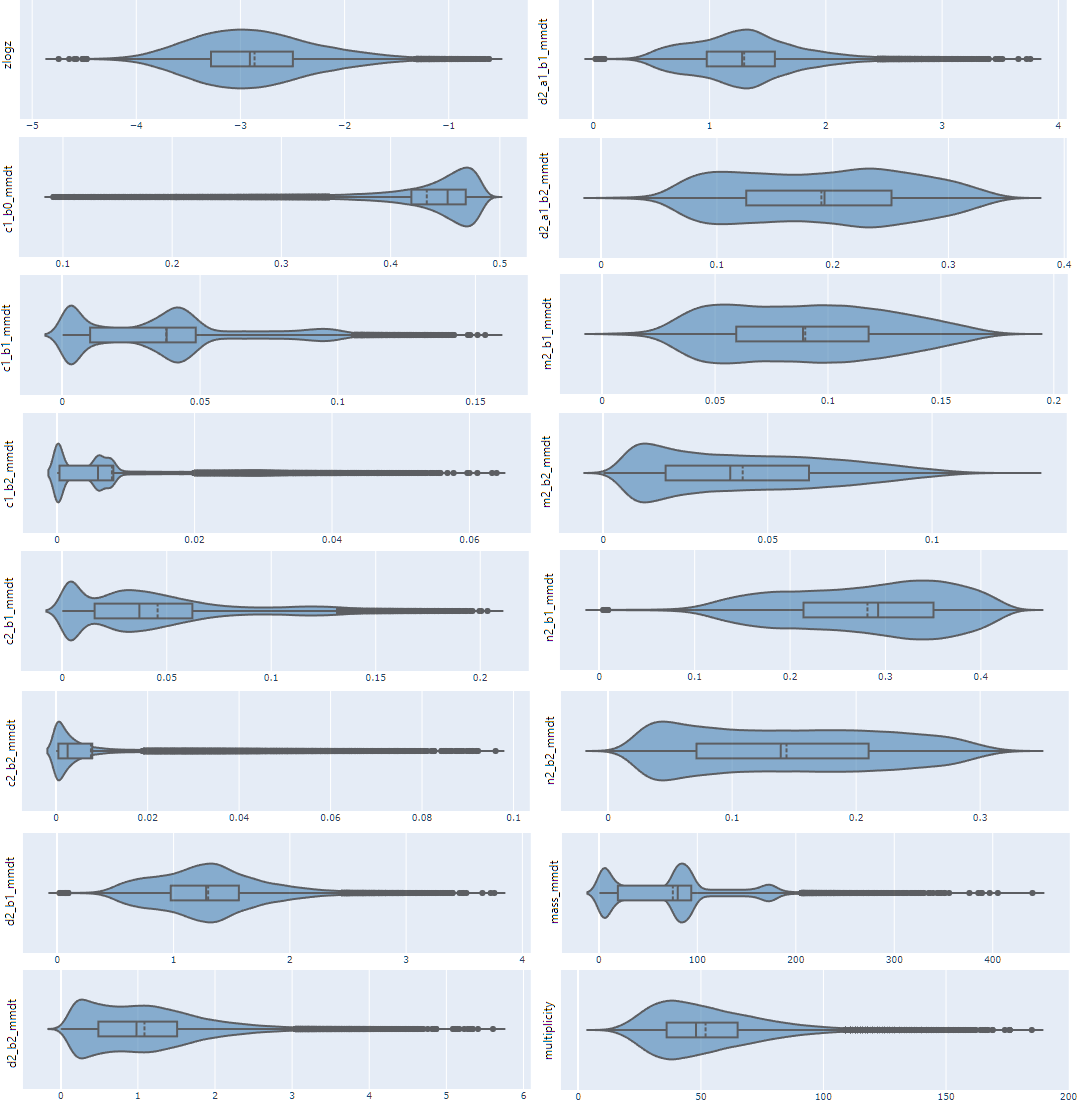
\includegraphics[trim={0cm 0cm 0cm 0cm}, width=1.0\textwidth, center]{background/distributions.png}
  \caption{Representation of the distributions of feature values in the HLF dataset.}
  \label{fig:distributions-hlf}
\end{figure}


\chapter{HLF dataset features distribution}
\begin{figure}[hpt!]
  \centering
  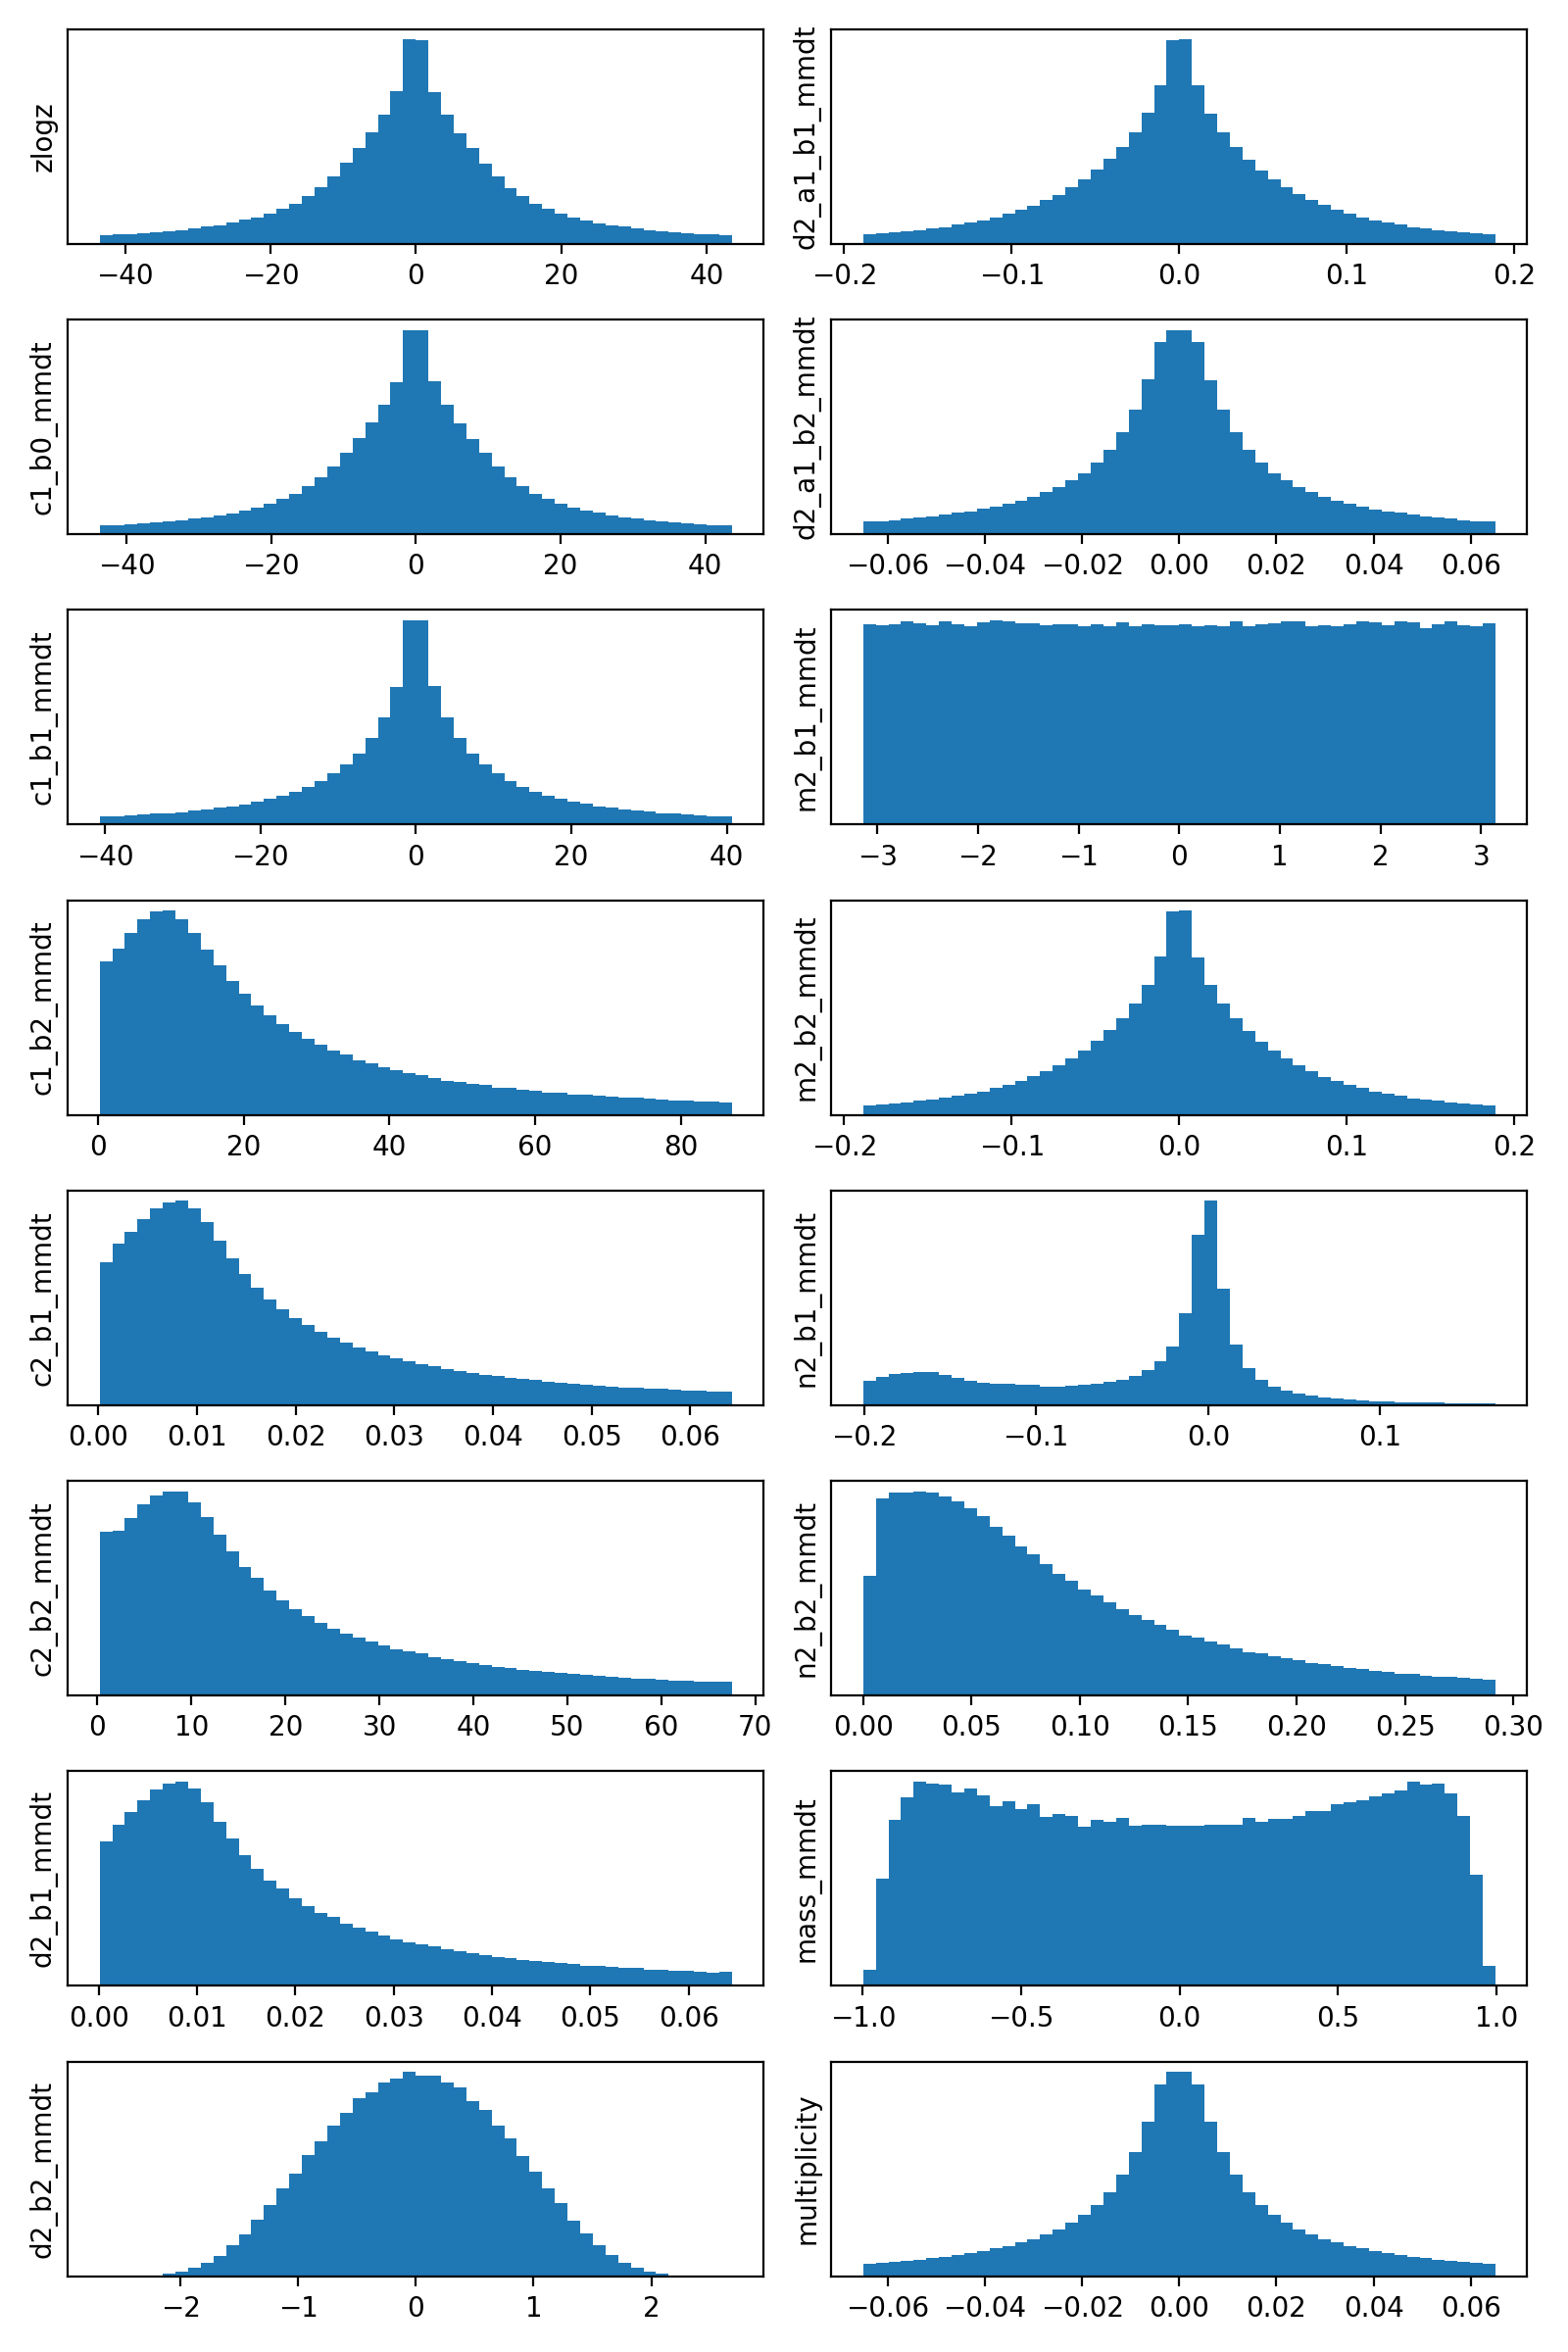
\includegraphics[trim={0cm 0cm 0cm 0cm}, width=0.7\textwidth, center]{../logs/constituent_distribution.png}
  \caption{Representation of the distributions of feature values in the constituent list dataset.}
  \label{fig:distributions-constituent}
\end{figure}

\end{appendices}

\listoftodos[Notes]

\end{document}